\documentclass[conference]{IEEEtran}
\usepackage[utf8]{inputenc}
\usepackage[pdftex]{hyperref}
\usepackage{algorithmic}
\usepackage{amssymb}
\usepackage{cite}
\usepackage{graphicx}

\hypersetup{
	colorlinks,
	linkcolor=blue,
	pdfauthor={Davide Pesavento \& Martina Astegno}
}

% correct bad hyphenation here
%\hyphenation{net-works}

\title{A dynamic audio routing system\\based on the RSSI of a Bluetooth device}% Audio streams routing based on the location of a passive Bluetooth device % Using the RSSI of a BT device to dynamically route audio streams % A proximity detection system for routing audio streams based on Bluetooth technology
\author{Davide~Pesavento, Martina~Astegno \\
	Università degli Studi di Padova \\
	Corso di Laurea Magistrale in Informatica \\
	\{dpesaven,mastegno\}@studenti.math.unipd.it
}


\begin{document}

\maketitle

\begin{abstract}
We present a prototype application that shows how the Bluetooth technology can be used to locate a person wearing a Bluetooth device (e.g. a smartphone) among a predefined set of rooms. The final aim is to reproduce an audio stream in one of these rooms and dynamically switch it from one speaker to another, according to the person's movements over time.
\end{abstract}

%\begin{IEEEkeywords} % normally used for peerreview paper
%Bluetooth, BlueZ, DBus, PulseAudio, audio routing, smartphone.
%\end{IEEEkeywords}

%\IEEEpeerreviewmaketitle

\section{Introduction}

\subsection{Bluetooth technology}
Bluetooth is an open specification for a radio system that provides the network infrastructure to enable short range wireless communication of data and voice. It comprises of a hardware component and a software component. The specification also describes usage models and user profiles for these models.
Bluetooth supports two kinds of links: Asynchronous Connectionless (ACL) links for data transmission and Synchronous Connection Oriented (SCO) links for audio/voice transmission. It uses Frequency Hopping Spread Spectrum (FHSS) to avoid any interference. A Bluetooth channel is divided into time slots each 625 micro second in length. The devices hop through these timeslots making 1600 hops per second. This trades bandwidth efficiency for reliability, integrity and security.
In figure~\ref{btstack} we can see the architecture of the Bluetooth protocol suite.

\begin{figure}[h]
\centering
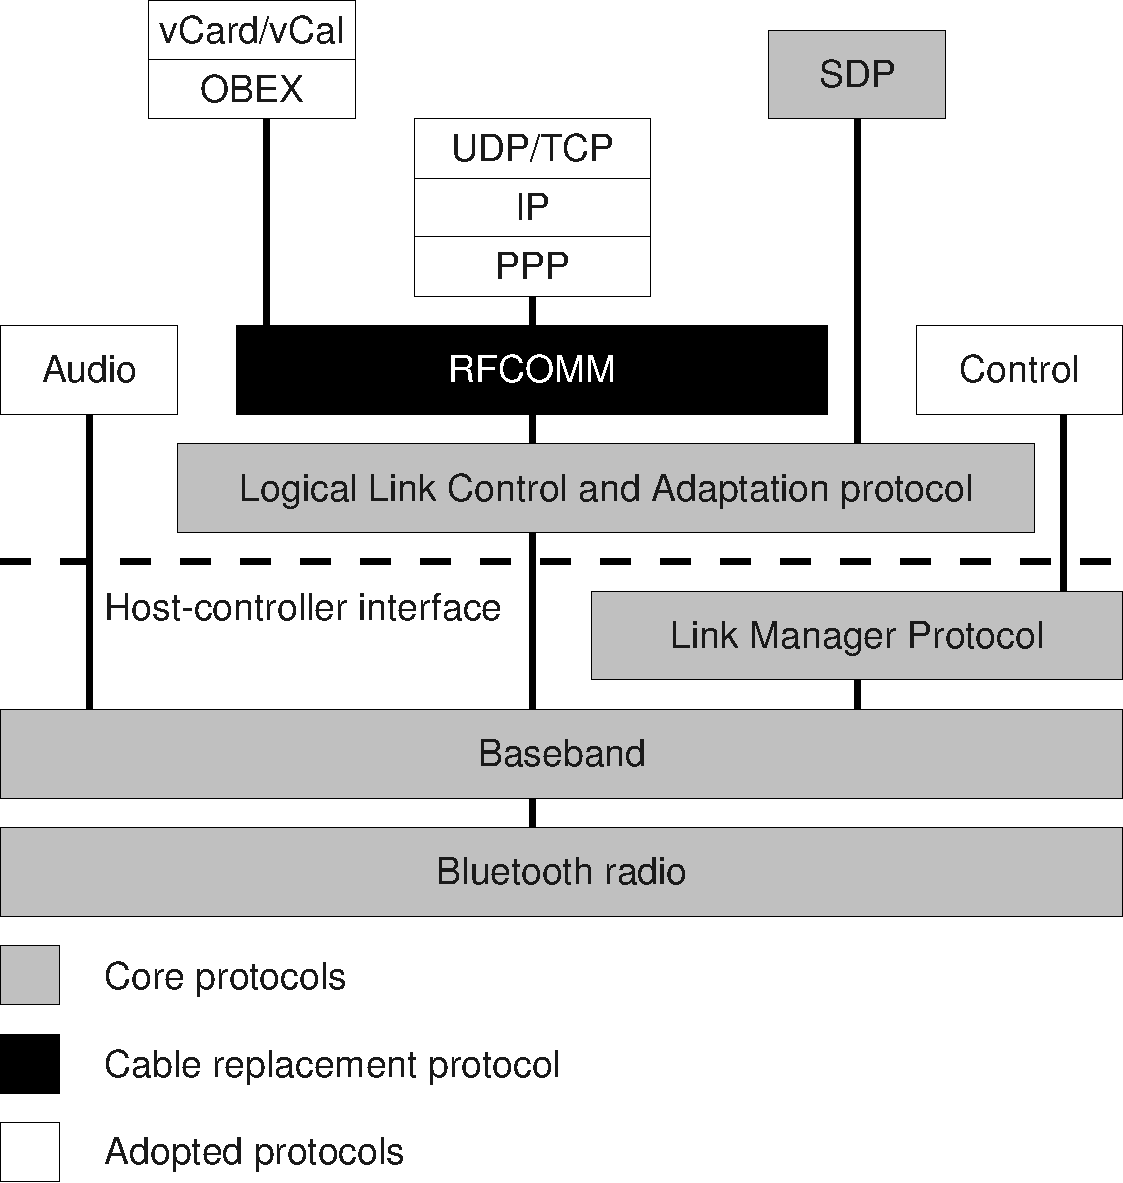
\includegraphics[width=0.9\columnwidth]{BTstack}
\caption{Bluetooth protocol stack}
\label{btstack}
\end{figure}

In our project we adopted a specific Bluetooth stack implementation, \textbf{BlueZ} version 4 or later, that provides support for the core Bluetooth layers and protocols. It is flexible, modular and efficient. Current versions of BlueZ consist of many separate modules:
\begin{itemize}
\item Bluetooth kernel subsystem core
\item L2CAP and SCO audio kernel layers
\item RFCOMM, BNEP, CMTP, HIDP kernel implementations
\item HCI UART, USB, PCMCIA and virtual device drivers
\item General Bluetooth and SDP libraries and daemon
\item Configuration and testing utilities
\item Protocol decoding and analysis tools
\end{itemize}

\subsection{PulseAudio server}
PulseAudio is a cross-platform, networked sound server. A sound server is basically a proxy for sound applications. It allows to do advanced operations on sound data as it passes between an application and the hardware. Things like transferring the audio to a different machine, changing the sample format or channel count and mixing several sounds into one are easily achieved using a sound server. PulseAudio is designed for Linux systems, but has been ported to Microsoft Windows, MacOS~X, Solaris, FreeBSD and other POSIX-compliant platforms. Figure~\ref{pa} depicts a high level overview of PulseAudio architecture.

\begin{figure}[h]
\centering
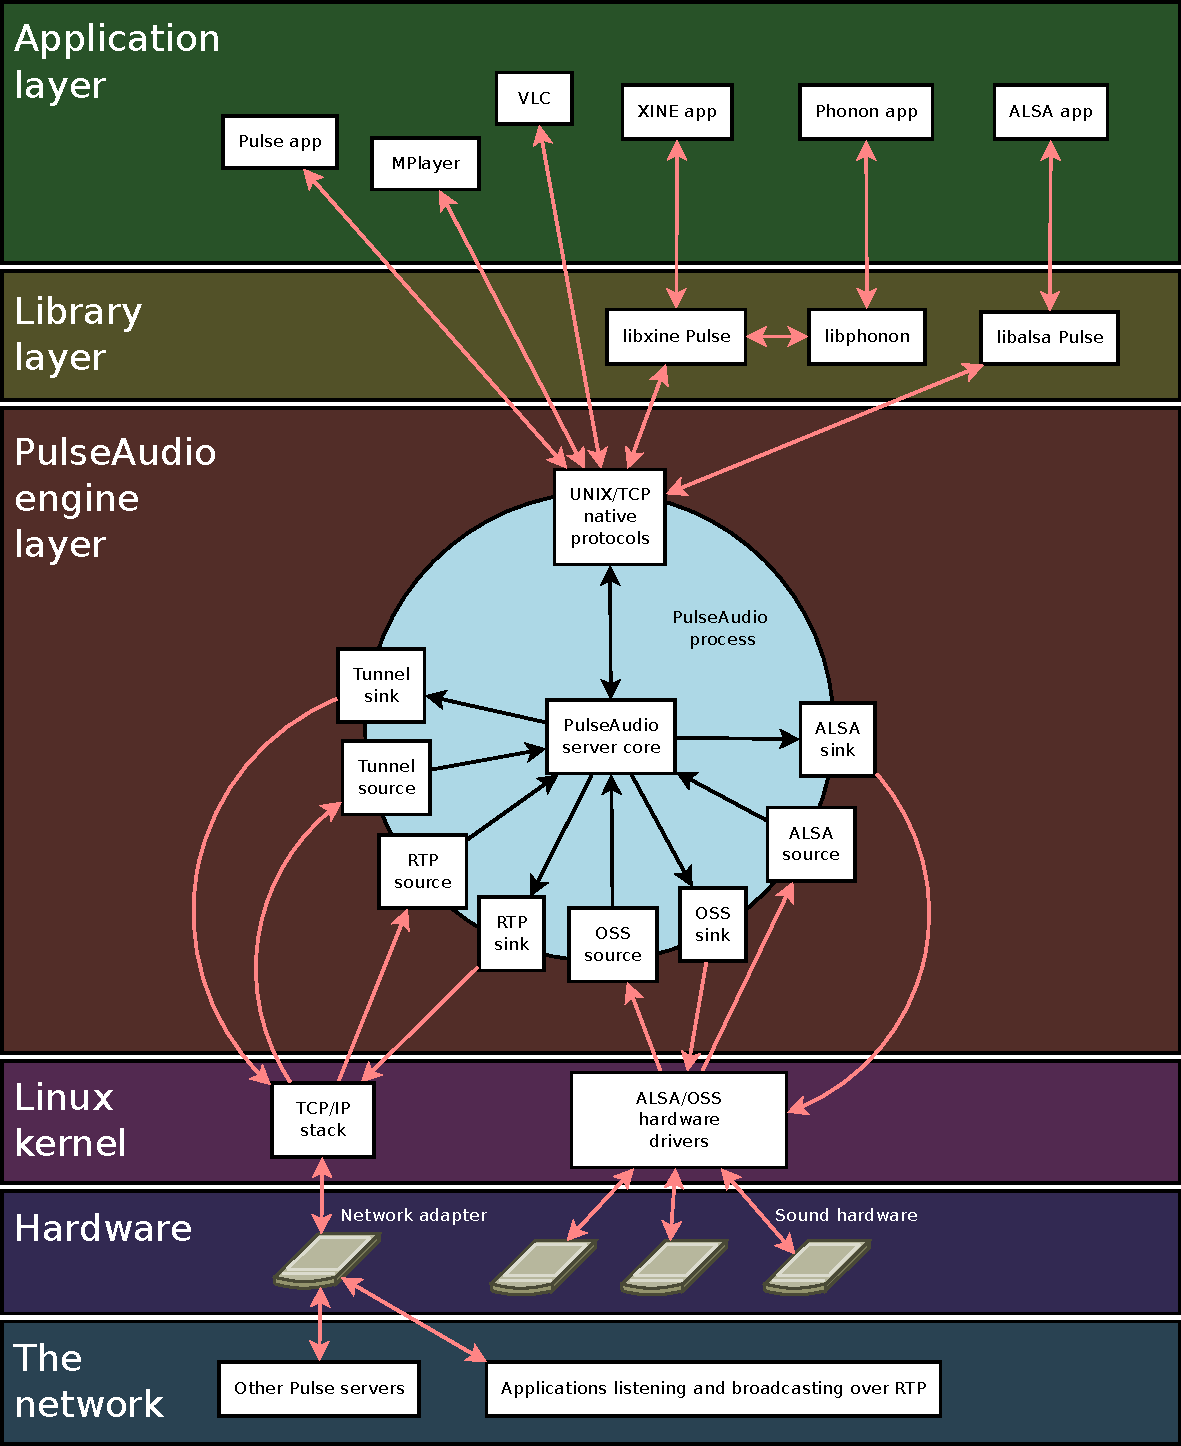
\includegraphics[width=\columnwidth]{PulseAudio}
\caption{High-level PulseAudio architecture}
\label{pa}
\end{figure}


\section{General architecture}

Our prototype consists of two different applications: \mbox{\textbf{Conductor}} and \textbf{Probe}.

\begin{figure*}
\centering
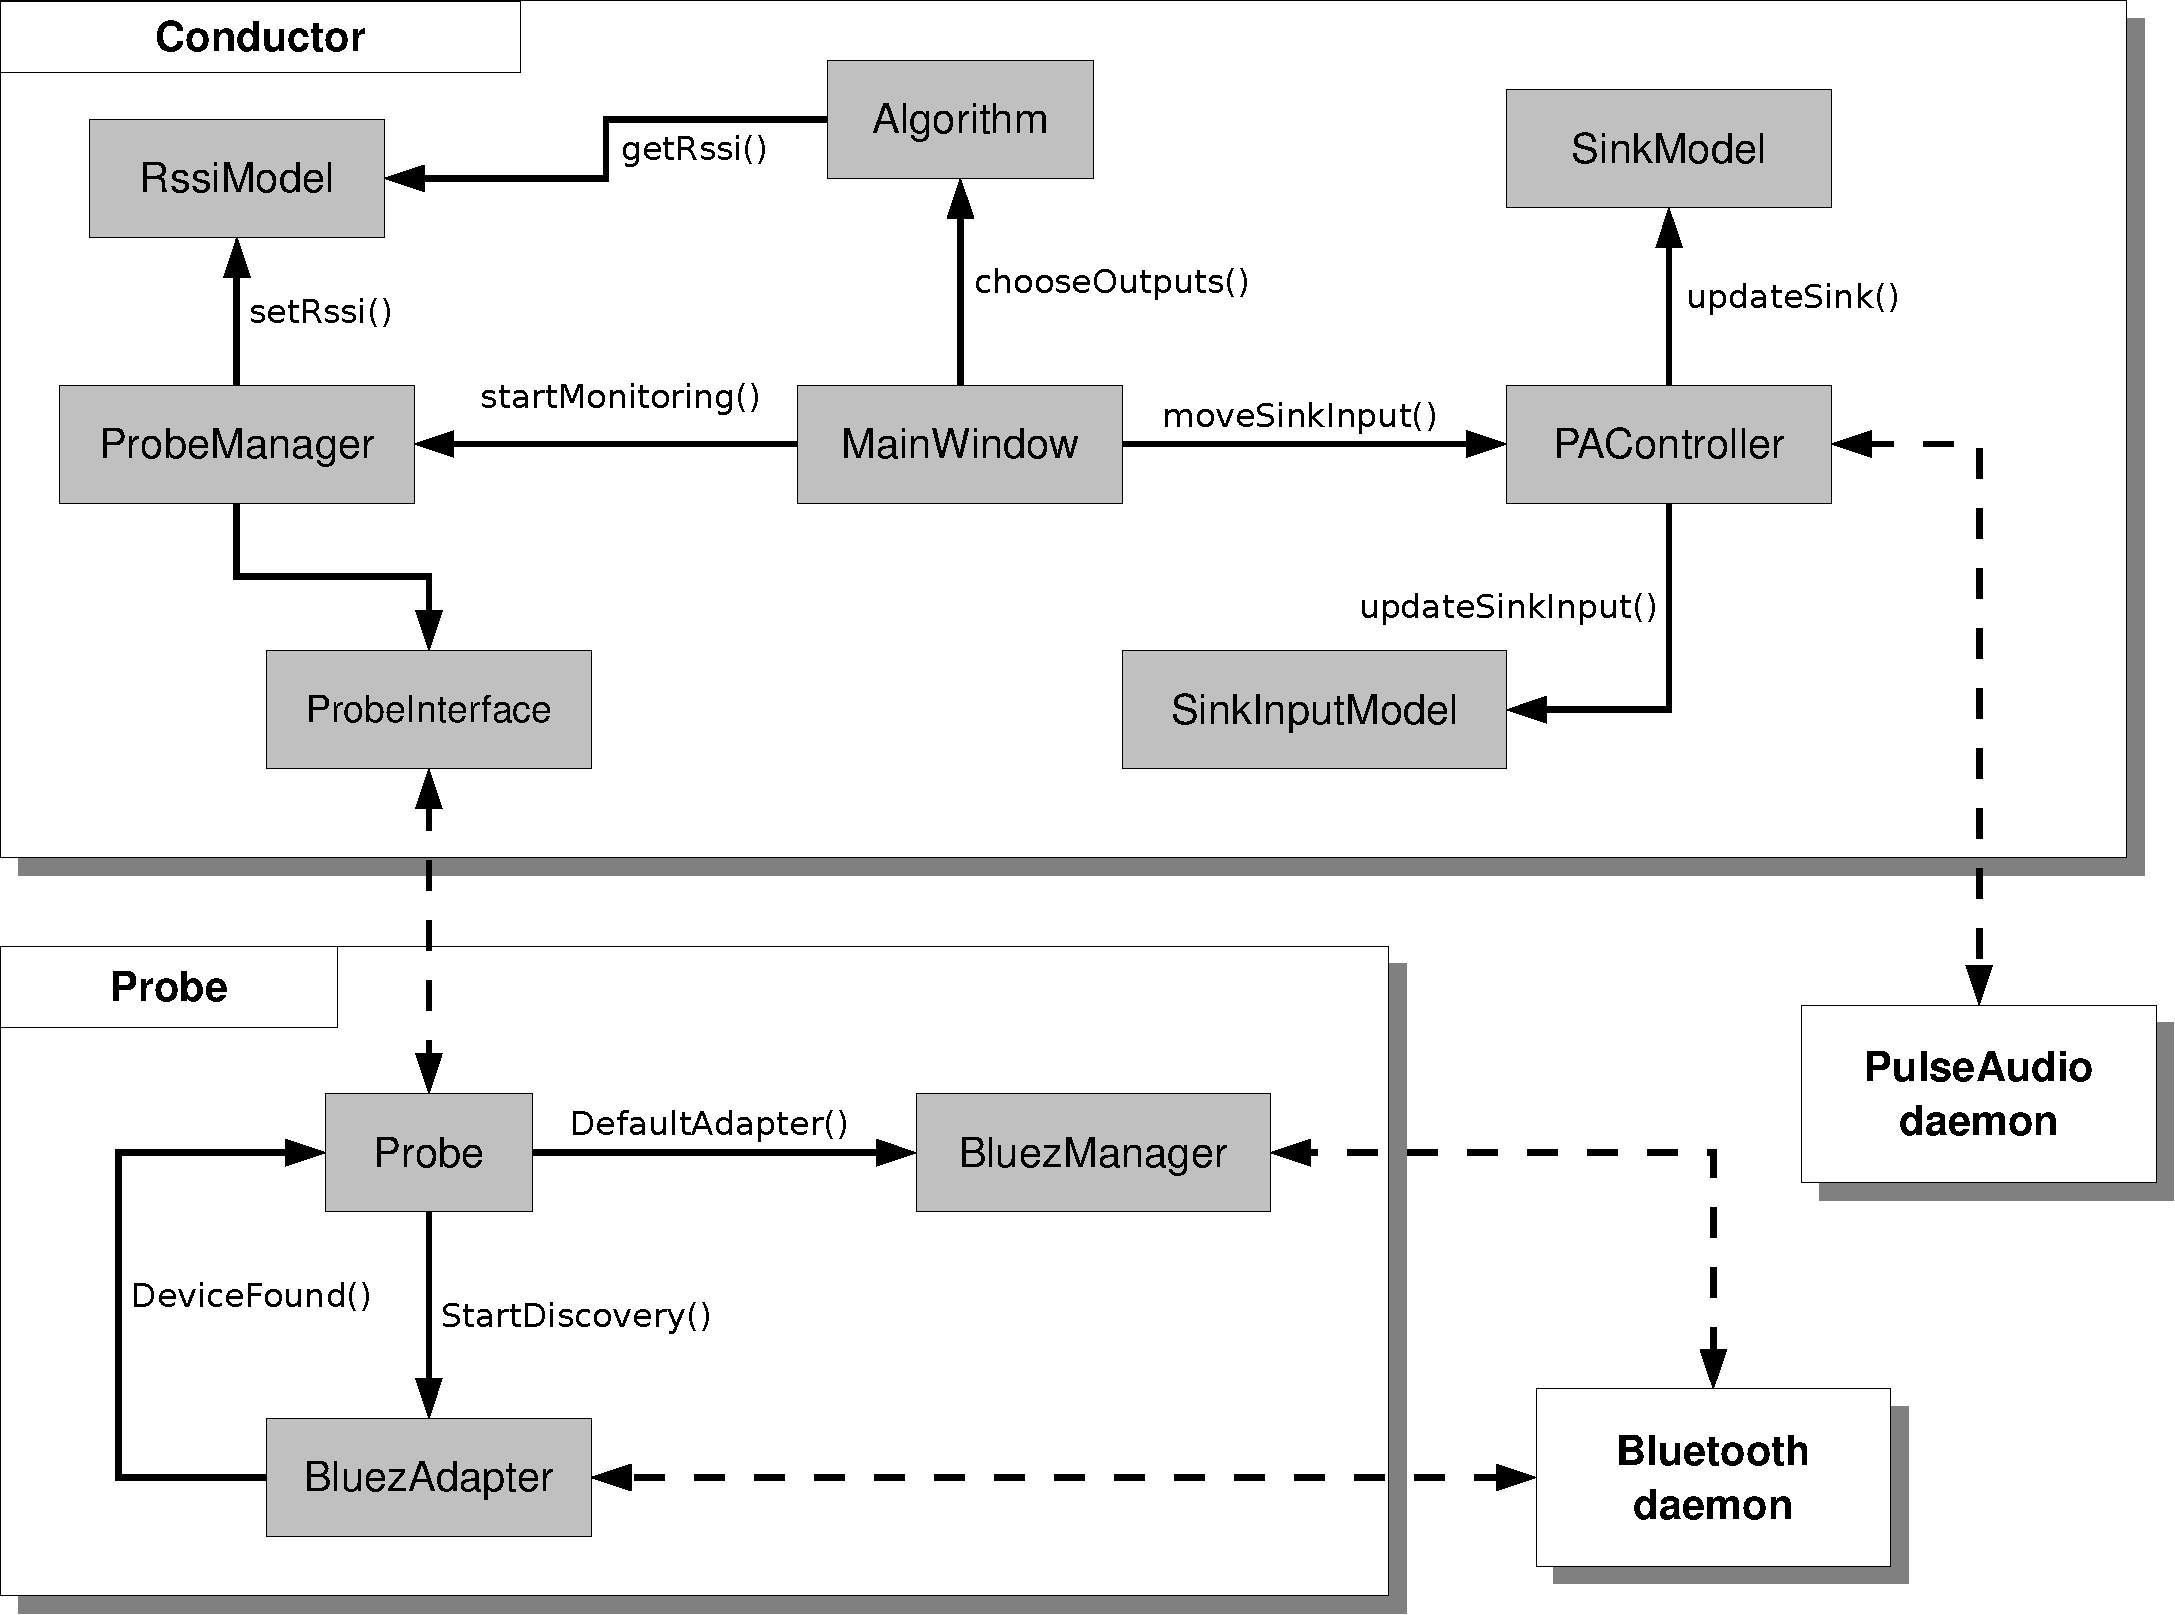
\includegraphics[width=0.85\textwidth]{Arch}
\caption{Main components and interactions between them}
\label{arch}
\end{figure*}

\subsection{Bluetooth module}
One of the most important components of the system is the Bluetooth module, that manages the RSSI values and communications between Bluetooth hosts and device. It is based on a simple and efficient application, named \texttt{probe} and associated to every Bluetooth adapter, that is able to interface with \textbf{BlueZ} through \textbf{DBus}. In detail, every Bluetooth adapter is modeled by the class \texttt{ProbeInterface}, that allows to start and stop a discovery done by the device and to update the RSSI values when a change occurs. All \texttt{ProbeInterface} objects are controlled by the class \texttt{ProbeManager} that monitors the device localization and stores the information about every \texttt{ProbeInterface} (e.g. the room name associated with the adapter).

\subsection{PulseAudio module}
The PulseAudio component has three main responsibilities:
\begin{itemize}
	\item \textbf{querying} the daemon for the list of available sinks and audio streams and keeping such information up-to-date;
	\item \textbf{loading} PulseAudio modules with the appropriate configuration and \textbf{unloading} them when they are no longer needed;
	\item \textbf{redirecting} an audio stream from one sink to another when requested by the application's logic.
\end{itemize}
All these operations are performed asynchronously. To keep track of in-flight operations, PulseAudio libraries return a reference-counted \texttt{pa\_operation} object for each of them.

Although the full introspection API is very powerful, it is also rather complex to use, being written in plain C and heavily relying on callbacks to implement asynchronous notifications. Therefore we developed a thin C++ layer on top of it, to simplify its usage by the rest of the application.

The two basic data structures at the bottom of PulseAudio, \texttt{pa\_sink} and \texttt{pa\_sink\_input}, are wrapped respectively by the classes \texttt{Sink} and \texttt{SinkInput}.
%\begin{itemize}
%	\item \texttt{pa\_sink}: it represents an ``exit point'' where the audio stream can be redirected;
%	\item \texttt{pa\_sink\_input}: it identifies a stream audio produced by a certain application.
%\end{itemize}

Asynchronous operations are wrapped in a similar way: each kind of operation is encapsulated by a different class, which hides all the details about how to submit that operation to the daemon and how to handle the result or a possible error. These classes are then organized into a simple hierarchy, with a common abstract base class (\texttt{PAOperation}) that exposes a unified interface to execute operations, without having to worry about their type.

The two most interesting \texttt{PAOperation} subclasses are:
\begin{itemize}
	\item \texttt{LoadModuleOperation}: loads a PulseAudio module to accomplish a specific task. In particular, our application uses the two following modules:
	\begin{itemize}
		\item \texttt{module-tunnel-sink} creates a new sink that forwards its input to the other end of the tunnel via a TCP connection; it requires a running PulseAudio daemon on the remote side.
		\item \texttt{module-combine} allows playing the same audio stream through two or more sinks simultaneously. A new virtual sink is allocated and all data written to it is forwarded to every connected sink.
	\end{itemize}
	\item \texttt{MoveOperation}: redirects a \texttt{SinkInput} from the current sink to the specified one.
\end{itemize}

On top of everything, class \texttt{PAController} is the façade for the whole module and provides a further level of abstraction. Internally it uses the classes described above, thus avoiding most of the complexity of interfacing with PulseAudio libraries directly. Its API is simple to use and consists mainly of these two methods:
\begin{itemize}
\item[$\vartriangleright$] \texttt{createTunnel(QByteArray server)}
\item[$\vartriangleright$] \texttt{moveSinkInput(SinkInput input, QList<QByteArray> speakers)}
\end{itemize}
The first method executes a \texttt{LoadModuleOperation} to create a tunnel sink towards the specified server. The second method redirects an arbitrary \texttt{SinkInput} to all the sinks corresponding to the specified list of speakers; this is accomplished using a \texttt{MoveOperation}, possibly preceded by the loading of an instance of \texttt{module-combine} if the list contains two or more speakers.

In order to implement these features, \texttt{PAController} has often the need to perform not just a single atomic operation but many of them. However these operations must usually be executed in a well-defined sequential order. This is quite difficult to achieve directly, due to the asynchronous nature of PulseAudio APIs. Therefore we designed a dedicated class (\texttt{PAOperationQueue}) which, while keeping an asynchronous design, is able to safely handle a queue of operations by submitting them only when all their dependencies have been satisfied, i.e. after the daemon notifies that all the operations on which they depend have been completed.

\subsection{Output selection algorithm}
This algorithm is the core of \textsl{Conductor}: it tries to figure out in which room the monitored device is currently located and, according to that, it selects the speakers that have to start reproducing sound.

The algorithm proceeds as follows. First of all, it obtains the latest RSSI value associated with each room using the method \texttt{RssiModel::getRssi()}. Then the values are sorted and a heuristics is applied to the highest ones. This heuristics takes into consideration the relative position of rooms, discarding any invalid combinations from the set of selected outputs (e.g. it does not make any sense to reproduce simultaneously in two rooms which are not contiguous). Finally, if the resulting set of rooms is different from the current one, the \texttt{outputsChanged} signal is emitted, allowing the rest of the application to react accordingly.

The following pseudo-code shows more precisely how the implemented algorithm works.

\vspace{2mm}
\textit{Short description of all variables involved in the algorithm}
\begin{itemize}
\item \texttt{adjacencyMap}: maps each room to the list of its adjoining rooms.
\item \texttt{best}: a set containing the rooms that have the first \texttt{maxSimultaneousSpeakers} highest RSSI values.
\item \texttt{curRooms}: the rooms where the audio stream is currently being played.
\item \texttt{maxRetries}: maximum number of retries (see \texttt{retryCount}); when exceeded the playback should be stopped.
\item \texttt{maxSimultaneousSpeakers}: maximum number of speakers that can be activated simultaneously.
\item \texttt{neighbors}: the set of rooms that are contiguous to at least one room in \texttt{curRooms}.
\item \texttt{outputs}: the new set of rooms chosen by the algorithm to reproduce the stream.
\item \texttt{retryCount}: an integer counter used to delay playback interruption when the device temporarily falls out of range.
\item \texttt{rssiMap}: maps each room to the last RSSI value received by the \textsl{Probe} located inside that room.
\end{itemize}

\vspace{2mm}
\textbf{\textit{Algorithm::chooseOutputs()}}
\begin{algorithmic}[1]
\STATE $retryCount \gets 0$
\STATE $outputs \gets \varnothing$
\STATE $best \gets \varnothing$

\STATE $sorted \gets sort(rssiMap)$
\FOR{$i = 1$ \textbf{to} $maxSimultaneousSpeakers$}
	\STATE $best \gets best \cup sorted[i]$
\ENDFOR

\IF{$best = \varnothing$ \textbf{and} $retryCount < maxRetries$}
	\STATE $retryCount \gets retryCount + 1$
	\STATE $sleep(updateInterval)$
	\STATE \textbf{goto} 4
\ENDIF

\STATE $neighbors \gets \varnothing$
\FORALL{$r \in curRooms$}
	\STATE $neighbors \gets neighbors \cup adjacencyMap[r]$
\ENDFOR

\STATE $outputs \gets best \cap neighbors$
\RETURN $outputs$
\end{algorithmic}

%\subsection{Tester}
%bisogna mettere che i dati sono precompilati, perchè non avevamo l'HW adatto che fornisse i lvalore di RSSI in seguito a d una inquiry.

\section{Operating system}

\subsection{Hardware requirements}
\label{hardware-requirements}
Before detailing the design of the prototype, we would like to point out some basic requirements for the project. Here, we propose a list and a description for the main ones.
\begin{itemize}
	\item{\textbf{Smartphone}:} the device used to determine the room in which the person is. For simplicity, we will assume that there is only one such device, but the prototype can trivially be extended to support an arbitrary number of devices.
	\item{\textbf{Central server}:} it runs the main control application and manages all the communication channels with the Bluetooth adapters.
\end{itemize}
Inside each room there must be available:
\begin{itemize}
	\item{a \textbf{Bluetooth adapter}:} it detects the received signal strength (RSSI) and sends it to the server through a very simple command-line application;
	\item{a \textbf{speaker}:} it lets out sound when the associate Bluetooth adapter is selected for playback.
\end{itemize}

\subsection{Configuration}
Before starting the application it is necessary to setup some parameters in the configuration file. The pieces of information that must be provided are:
\begin{itemize}
\item \texttt{maxRetries}: a threshold useful when the device is out of range to decide if the playback has to be stopped or not.
\item \texttt{maxSimultaneousSpeakers}: the maximum number of speakers activated at the same time.
\item \texttt{probesAddresses}: the IP addresses of Probes associated with each room.
\item \texttt{roomsNames}: the names associated with each room.
\item \texttt{roomsTopology}: it describes the relative localization of each room. %respect to each other.
\item \texttt{updateInterval}: the amount of time (in milliseconds) after which the algorithm is repeated in a cyclic way.
\end{itemize}

\subsection{Runtime behavior}
%description about components interaction
In this section we will describe the system runtime behavior, showing how different components can interact and how the RSSI values are used to control the audio stream.
Periodically, through an inquiry, the Probes will obtain the RSSI values detected with respect the smartphone. If the difference between the new and the preceeding RSSI values is higher than a fixed threshold, the Probes transmit them to the main application on the central server. This operation is executed at regular intervals to estimate in which room the person with the device is. If this is different from the room in which the playback is currently running, this information is comunicated to the \texttt{PAController} and a request is sent to move the selected audio stream to the speaker associated with the new room. At this point there are two possible scenarios according to the number of speakers that have to be activated:
\begin{itemize}
	\item one speaker: the audio stream is directly redirected to the respective tunnel;
	\item two or more speakers: it is necessary to load the combine-module (PulseAudio module), that creates a virtual sink to reproduce the stream through all the connected sinks (slaves).
\end{itemize}

\section{Experiments Evaluation}
To verify the correct system functioning we executed specific tests in a simulated environment. To perform tests we used two notebooks that act as speakers, for two different ``virtual'' rooms, connected via Ethernet. In the main interface application, that runs on one of these two machines, there are three areas containing:
\begin{itemize}
	\item the complete list of available sink inputs with the corresponding identifiers;
	\item the complete list of sinks detected with the corresponding IP addresses and identifiers;
	\item the list of rooms with an editable field, with the corresponding RSSI values, for each ones.
	\end{itemize}

When the application, in testing mode starts, the sound is reproduced throught the speaker specified as default parameter. The user can move the audio stream from a computer to the other (or play simultaneously) changing the RSSI values associated with each ones. The stream is redirected to the room with an RSSI value different by \texttt{NULL}. If there isn't an RSSI value equals to \texttt{NULL} the sound is reproduced throught both speakers. Finally if both RSSI values are equal to \texttt{NULL}, the playback occurs throught the last speaker that has reproduced the sound.


\section{Future work}
In this section we examine some possible future extensions of the project.

\subsection{Real-world testing}
The prototype has been tested through an additional user interface that allows to simulate a person's movements. This interface exposes a monitor with an editable input box for each room. By interacting with it, the user is able to insert an arbitrary RSSI value to simulate his movements among the rooms (the higher the value, the closer he is to the corresponding room). However this is just a simulation, thus the overall system behavior might be slightly different in the real-world case.

In order to improve the consistency and the reliability of test results, it is therefore advisable to perform a more thorough testing session in a real-world scenario. We could not do that due to the lack of a sufficient number of Bluetooth adapters satisfying the hardware requirements outlined in section~\ref{hardware-requirements}.

A more realistic testing phase could also have highlighted some shortcomings of the current algorithm and would have enabled us to fine-tune it to meet the initial expectations for the project.

\subsection{Multiple monitored devices}
In section~\ref{hardware-requirements} we assumed that there is only one device to monitor. However we believe that extending the system to be able to locate multiple devices would be a major feature. This entails the necessity of evaluating how different devices could interact, and will eventually require the development of a policy to handle conflicts between them. Once a solution to this potential issue has been found, modifying the current implementation should be trivial because the prototype has already been designed with this extension in mind, so the code is already quite generic and makes very few assumptions about the number of monitored devices.

\subsection{Lightweight control application on device}
Currently the device is only used to locate the person wearing it. It would be interesting to develop a mobile application to give the user a certain degree of control on audio streams. For instance, with this new feature, he should be able to adjust the volume and pause or stop the playback. A further improvement could be an interface to navigate through the playlist, i.e. choose a specific song or skip to the previous/next track.


\section{Conclusions}
TODO


\begin{thebibliography}{1}
\bibitem{PulseAudio}
	PulseAudio Sound Server,\\
	\url{http://www.pulseaudio.org/}
\bibitem{PulseaudioDoc}
	PulseAudio API documentation,\\
	\url{http://0pointer.de/lennart/projects/pulseaudio/doxygen/}
\bibitem{BlueZ}
	BlueZ: the official Linux Bluetooth protocol stack,\\
	\url{http://www.bluez.org/}
\end{thebibliography}

\end{document}
